%%%%%%%%%%%%%%%%%%%%%%%%%%%%%%%%%%%%%%%%%%%%%%%%%%%%%%%%%%%%%%%%%%%%%%%%%%%%%%%%
% TUM-Vorlage: Präsentation - Beispiele
%%%%%%%%%%%%%%%%%%%%%%%%%%%%%%%%%%%%%%%%%%%%%%%%%%%%%%%%%%%%%%%%%%%%%%%%%%%%%%%%


%%%%%%%%%%%%%%%%%%%%%%%%%%%%%%%%%%%%%%%%%%%%%%%%%%%%%
%% Folie: Gültigkeit der Masterfolien              %%
%%%%%%%%%%%%%%%%%%%%%%%%%%%%%%%%%%%%%%%%%%%%%%%%%%%%%

%%%%%%%%%%%%%%%%%%%%%%%%%%%%%%%%%%%%%%%%%%%%%%%%%%%%%
%% Folie: Grundlage der Masterfolien               %%
%%%%%%%%%%%%%%%%%%%%%%%%%%%%%%%%%%%%%%%%%%%%%%%%%%%%%

%%%%%%%%%%%%%%%%%%%%%%%%%%%%%%%%%%%%%%%%%%%%%%%%%%%%%
%% Folie: 2-zeilige Überschrift                    %%
%%%%%%%%%%%%%%%%%%%%%%%%%%%%%%%%%%%%%%%%%%%%%%%%%%%%%


%%%%%%%%%%%%%%%%%%%%
%%%%%%%%%%%%%%%%%%%%
\begin{frame}
    \shiftedframetitle{Content}

    \begin{enumerate}
    \item Shallow Water Equations model \vspace{0.5cm}
    \item Scope of this thesis\vspace{0.5cm}
    \item Tools\vspace{0.5cm}
    \item Current status\vspace{0.5cm}
    \item Next steps
    \end{enumerate}



\end{frame}
\clearpage


%%%%%%%%%%%%%%%%%%%%
%%%%%%%%%%%%%%%%%%%%
\begin{frame}
    \shiftedframetitle{Shallow Water Equations (SWE) model}
\vspace{-3mm}
\begin{itemize}
\item<2-> $3D$ Navier-Stokes Equations for \textbf{incompressible inviscid} flow (\ref{ns}) and \textbf{mass continuity law} (\ref{cont})
\vspace{0.5cm}
\begin{align}
\frac{\partial u}{\partial t} + u\frac{\partial u}{\partial x} + v\frac{\partial u}{\partial y} + w\frac{\partial u}{\partial z} &= - \frac{\partial p}{\partial x} \nonumber \\[0.8cm]
\frac{\partial v}{\partial t} + u\frac{\partial v}{\partial x} + v\frac{\partial v}{\partial y} + w\frac{\partial v}{\partial z}&= - \frac{\partial p}{\partial y} \label{ns} \\[0.8cm]
\frac{\partial w}{\partial t} + u\frac{\partial w}{\partial x} + v\frac{\partial w}{\partial y} + w\frac{\partial w}{\partial z} &= - \frac{\partial p}{\partial z} + g \nonumber\\[1.5cm]
\frac{\partial u}{\partial x} + \frac{\partial v}{\partial y} + \frac{\partial w}{\partial z} &= 0 \label{cont}
\end{align}
\end{itemize}
\end{frame}
\clearpage


%%%%%%%%%%%%%%%%%%%%
%%%%%%%%%%%%%%%%%%%%
\begin{frame}
    \shiftedframetitle{Shallow Water Equations (SWE) model {\small(cont.)}}
\vspace{-3mm}
\begin{itemize}
\setlength\itemsep{2em}
\item<1-> \textbf{First assumption}: $L \gg H$, from mass continuity (\ref{cont})
\begin{align*}
\color{TUMOrange}\underbrace{\color{black}\frac{\partial u}{\partial x} + \frac{\partial v}{\partial y}}_{\approx \frac{2U}{L}} \color{black} + \color{TUMOrange}\underbrace{\color{black}\frac{\partial w}{\partial z}}_{\myTUMorange{\approx \frac{W}{H}}} &= 0
\end{align*}

leading to \myTUMorange{$u,v\gg w$}
\item<2-> \textbf{Second assumption}: \myTUMdarkblue{vertical momentum exchange} is \myTUMdarkblue{negligible}. Then, NS equation \myTUMdarkblue{vertical component} modifies to
\begin{align}
\color{TUMDarkBlue}\underbrace{\color{black}\frac{\partial w}{\partial t} + u\frac{\partial w}{\partial x} + v\frac{\partial w}{\partial y} + w\frac{\partial w}{\partial z}}_{\myTUMdarkblue{0}}  \color{black} = - \frac{\partial p}{\partial z} + g \nonumber\\[0.5cm]
\myTUMdarkblue{0} \myTUMdarkblue{= - \frac{\partial p}{\partial z} + g} \label{press}
\end{align}
\item<3->[]
This provides a \myTUMdarkblue{solution for the pressure} as a function of the sea floor elevation and water level
\end{itemize}
\end{frame}
\clearpage



%%%%%%%%%%%%%%%%%%%%
%%%%%%%%%%%%%%%%%%%%
\begin{frame}
    \shiftedframetitle{Shallow Water Equations (SWE) model {\small(cont.)}}
\vspace{-3mm}
\begin{itemize}
\item<1-> \myTUMorange{Depth-averaged integration} on the continuity equation \ref{cont}
\begin{align}
\myTUMorange{\int_{b_0}^{b_0 + h }} (\frac{\partial u}{\partial x} + \frac{\partial v}{\partial y} + \myTUMorange{\frac{\partial w}{\partial z}})\ \myTUMorange{dz} &= 0 \nonumber \\[0.8cm]
\myTUMorange{\frac{\partial h}{\partial t}} + \frac{\partial \myTUMorange{h}u}{\partial x} + \frac{\partial \myTUMorange{h}v}{\partial y} &= 0
\end{align}
\vspace{0.5cm}
\item<2->\myCRed{\textit{Leibnitz Integral Rule}} $+$ \myCRed{depth-averaged integration} on the momentum equation $+$ kinematic \myCRed{BCs} on surface \cite{depthAv} $+$ \myTUMdarkblue{(\ref{press})}
\begin{align}
\frac{\partial \myCRed{hu}}{\partial t} + \frac{\partial}{\partial x}(\myCRed{hu^2} + \myTUMdarkblue{\frac{1}{2} g h^2}) + \frac{\partial \myCRed{huv}}{\partial y} &= \myTUMdarkblue{- gh\frac{\partial b}{\partial x}} \\[0.8cm]
\frac{\partial \myCRed{hv}}{\partial t} + \frac{\partial \myCRed{huv}}{\partial x} + \frac{\partial}{\partial y}(\myCRed{hv^2} + \myTUMdarkblue{\frac{1}{2} g h^2})&= \myTUMdarkblue{- gh\frac{\partial b}{\partial y} }
\end{align}
\end{itemize}
\end{frame}
\clearpage

%%%%%%%%%%%%%%%%%%%%
%%%%%%%%%%%%%%%%%%%%
\begin{frame}
    \shiftedframetitle{Shallow Water Equations (SWE) model {\small(cont)}}
\vspace{-2mm}

\begin{columns}
\begin{column}{0.4\textwidth}
\begin{itemize}
\item<1->[] SWE model can be represented in a {\color{TUMBlauDunkel}matrix} form \dots
% derived from mass and momentum conservation laws, and depth averaging \dots %also derived by vertical averaging from the 3d incompressible ns eqs
\item<2->[]
\begin{align*}
\vspace{-15pt}
\begin{bmatrix}[1.3]
\myTUMdarkblue{h}\\
\myTUMdarkblue{hu}\\
\myTUMdarkblue{hv}\\
\end{bmatrix}_t \ + \
\begin{bmatrix}[1.0]
hu\\
hu^2 + \frac{1}{2}gh^2\\
huv\\
\end{bmatrix}_x\ &+ \
\begin{bmatrix}[1.0]
hv\\
huv\\
hv^2 + \frac{1}{2}gh^2\\
\end{bmatrix}_y =
\begin{bmatrix}[1.0]
0\\
-gh\ b_x\\
-gh\ b_y
\end{bmatrix}\\[2em]
\bar{q} = &\begin{bmatrix}[1.3]
\myTUMdarkblue{h}\\
\myTUMdarkblue{hu}\\
\myTUMdarkblue{hv}
\end{bmatrix}
\begin{matrix}[1.0]
\text{\hspace{-3em}\myTUMdarkblue{$\rightarrow\ $\textit{height}}}\\
\text{\hspace{-2pt}\myTUMdarkblue{$\rightarrow\ $\textit{dicharge in x}}} \\
\text{\hspace{5pt}\myTUMdarkblue{$\rightarrow\ $\textit{discharge in y}}}
\end{matrix}
\end{align*}
\vspace{2pt}
\item<4->[]
\begin{align*}
\qquad \qquad \frac{\partial \bar{q}}{\partial t} + \dfrac{\partial \bar{F}(q)}{\partial x} + &\frac{\partial \bar{G}(q)}{\partial y} = S(h,x,y,t)
\end{align*}
\end{itemize}

\end{column}
\begin{column}{0.6\textwidth}  %%<--- here
\begin{itemize}[leftmargin=*]
\item<3->[]
\vspace{2cm}
\begin{center}
\begin{figure}
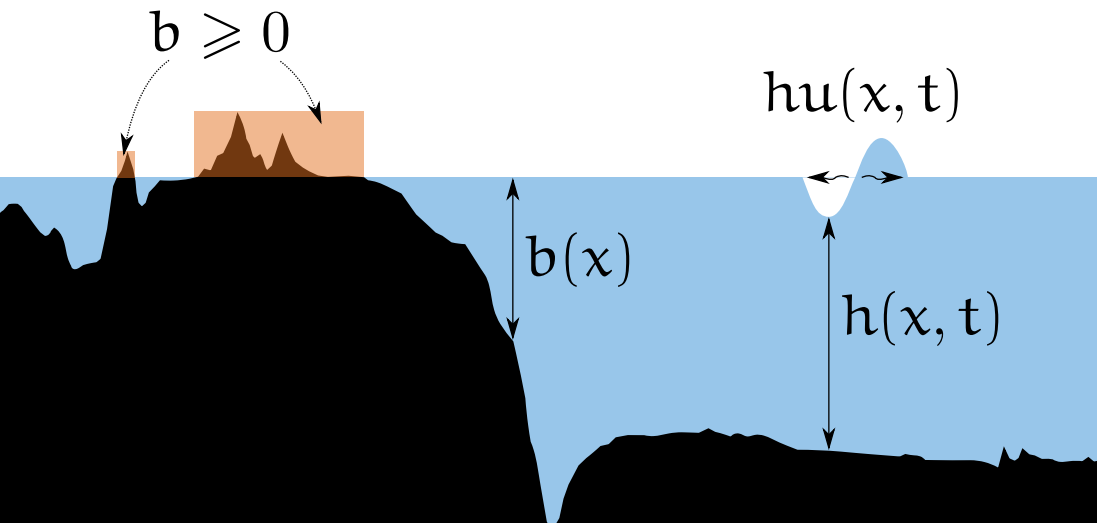
\includegraphics[scale=0.32]{./Resources/Images/swe_edit.png}%
\caption{SWE variables schematic \footnotemark}
\label{fig:swechemedit}
\end{figure}
\end{center}
\end{itemize}
\end{column}
\end{columns}
\vspace{-2em}
%\footnotemark
\footnotetext{\url{https://www5.in.tum.de/SWE/lugano2013/swe_anatomy.pdf}}

\end{frame}
\clearpage


%%%%%%%%%%
%%%%%%%%%%

%\begin{frame}
%    \shiftedframetitle{Shallow Water Equations (SWE) model {\small(cont)}}
%\vspace{-2mm}
%\begin{multicols}{2}
%\begin{itemize}
%\item<1->[] SWE model can be represented in a {\color{TUMBlauDunkel}matrix} form \dots
%% derived from mass and momentum conservation laws, and depth averaging \dots %also derived by vertical averaging from the 3d incompressible ns eqs
%\item<2->[]
%\begin{align*}
%\vspace{-15pt}
%\begin{bmatrix}[1.3]
%\myTUMdarkblue{h}\\
%\myTUMdarkblue{hu}\\
%\myTUMdarkblue{hv}\\
%\end{bmatrix}_t \ + \
%\begin{bmatrix}[1.0]
%hu\\
%hu^2 + \frac{1}{2}gh^2\\
%huv\\
%\end{bmatrix}_x\ &+ \
%\begin{bmatrix}[1.0]
%hv\\
%huv\\
%hv^2 + \frac{1}{2}gh^2\\
%\end{bmatrix}_y =
%\begin{bmatrix}[1.0]
%0\\
%-gh\ b_x\\
%-gh\ b_y
%\end{bmatrix}\\[1em]
%\bar{q} = &\begin{bmatrix}[1.3]
%\myTUMdarkblue{h}\\
%\myTUMdarkblue{hu}\\
%\myTUMdarkblue{hv}\\
%\end{bmatrix}
%\begin{matrix}[1.0]
%\text{\hspace{-3em}\myTUMdarkblue{$\rightarrow\ $\textit{height}}}\\
%\text{\hspace{-2pt}\myTUMdarkblue{$\rightarrow\ $\textit{dicharge in x}}} \\
%\text{\hspace{5pt}\myTUMdarkblue{$\rightarrow\ $\textit{discharge in y}}}
%\end{matrix}\\[2em]
%\frac{\partial \bar{q}}{\partial t} + \dfrac{\partial \bar{F}(q)}{\partial x} + &\frac{\partial \bar{G}(q)}{\partial y} = S(h,x,y,t) \\[3em]
%\end{align*}
%%\end{itemize}
%
%\vfill\columnbreak
%\vspace*{0.4cm}
%%\begin{itemize}
%\item<3->[]
%\begin{figure}
%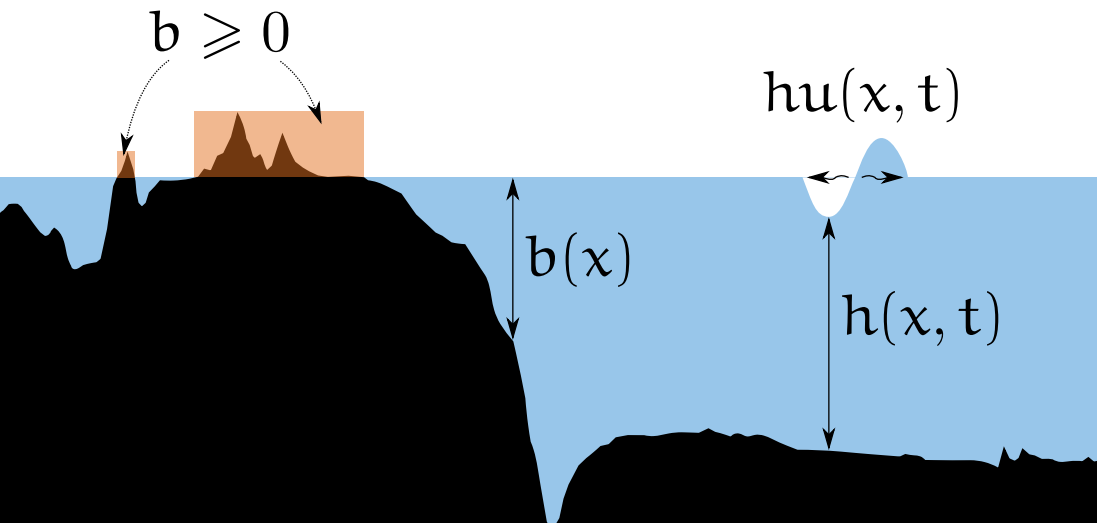
\includegraphics[scale=0.32]{./Resources/Images/swe_edit.png}%
%\caption{SWE variables schematic \footnote{\url{https://www5.in.tum.de/SWE/lugano2013/swe_anatomy.pdf}}}
%\label{fig:swechem}
%\end{figure}
%\end{itemize}
%\end{multicols}
%\end{frame}
%\clearpage

%%%%%%%%%%%%%%%%%%%%
%%%%%%%%%%%%%%%%%%%%
\begin{frame}
    \shiftedframetitle{Shallow Water Equations (SWE) model {\small(final)}}
\begin{itemize}
\setlength\itemsep{2em}
\item<1->[] The \textbf{\myTUMgreen{Shallow Water Equations}} \dots
\item<2-> \myTUMgreen{neglect vertical velocity}:  $ W \ll U,V $, horizontal distances $L$ $\gg$ vertical distance $H$
\item<3-> provide a \myTUMgreen{solution} for the \myTUMgreen{pressure}
\item<4-> simplify \myTUMgreen{$3D$} Navier-Stokes \myTUMgreen{to} a \myTUMgreen{$2D$} system of equations
\item<5-> represent a \myTUMgreen{hyperbolic PDE} system $\rightarrow$ \myTUMgreen{Riemann} Problem and \myTUMgreen{FVM}
\item<6-> Applications: {\small \myTUMgreen{Free surface} flows around structures, tsunamis prediction, atmospheric flows, \dots}
\end{itemize}
\end{frame}
\clearpage


%%%%%%%%%%%%%%%%%%%%%%%%%%
%%%%%%%%%%%%%%%%%%%%%%%%%%

\begin{frame}
\shiftedframetitle{Scope of this thesis}

\begin{multicols}{2}
\begin{itemize}
\item<2->[]
 \hspace{0.35\columnwidth}{\large\textbf{Background}}
 \vspace{3em}
 \begin{itemize}
  \setlength\itemsep{2em}
  \item  full description of \myTUMdarkblue{\textit{shallowFOAM}}  solver for \myTUMdarkblue{$2D$} SWE \cite{mintgen}
 \item  \myTUMdarkblue{coupling $2D$} SWE and \myTUMdarkblue{$3D$} RANS solvers $\rightarrow$ development of \textit{shallowInterFOAM} \cite{mintgen}
 \item B.Sc. Christiaan Osse implemented \cite{mintgen} with \myTUMdarkblue{\textit{preCICE}}
 \end{itemize}

\vfill\columnbreak

\item<3->[]
\hspace{0.35\columnwidth}{\large\textbf{Goals}}
\vspace{3em}
 \begin{itemize}

 \item<4-> \myCRed{Extend} \cite{mintgen} coupling ($2D$ $\leftrightarrow$ $3D$) as a \myCRed{flexible} approach to SWE solvers\\[2em]
 \item<5-> Test Case: $2D$ SWE solver \& OpenFOAM\\[2em]
 \item<6-> \myCRed{Coupling} \& \myCRed{Mapping} data from/to all setups: \vspace{0.4cm}
\begin{table}[]
\begin{tabular}{|lll|}\hline
$2D$ SWE       & $\rightarrow$ & $2D$ SWE       \\ \hline
$2D$ SWE       & $\rightarrow$ & $3D$ OpenFOAM \\ \hline
$3D$ OpenFOAM & $\rightarrow$ & $2D$ SWE       \\ \hline
$3D$ OpenFOAM & $\rightarrow$ & $3D$ OpenFOAM \\ \hline
\end{tabular}
\caption{Mapping setups}
\label{table:1}
\end{table}
\item<7-> \textbf{\textit{\myCRed{Extend preCICE} adapter for handling $2D\leftrightarrow3D$ domains}}
\end{itemize}
\end{itemize}
\end{multicols}


\end{frame}


%%%%%%%%%%%%%%%%%%
%%%%%%%%%%%%%%%%%%

\begin{frame}
	\shiftedframetitle{Tools}

\begin{multicols}{2}
\begin{itemize}
 \setlength\itemsep{10pt}

\item<2->[]
\textbf{Shallow Water Equations Solver - {\small Wave-propagation method.}}
\begin{itemize}
\vspace{5pt}
 \setlength\itemsep{6pt}
\item Modified Wave-Propagation Method $\rightarrow$ \myCRed{\textit{F-Wave}} \cite{levequeArticle}
\item Developed at SCCS\footnote{\url{https://github.com/TUM-I5/SWE}}
\item Written in \myCRed{C++}
\item \myCRed{$2D$}
\end{itemize}

\item<3->[]
\textbf{\textit{interFoam}\footnote{\url{https://openfoamwiki.net/index.php/InterFoam}} - {\small OpenFOAM Multiphase Navier-Stokes Solver}}
\begin{itemize}
\vspace{5pt}
 \setlength\itemsep{6pt}
\item \myCRed{VoF} (Volume of Fluid) method $\rightarrow$ phase-fraction interphase approach \myCRed{$\rho=\alpha\rho_1 + (1-\alpha)\rho_2$}
\item immiscible fluids (2-Phase)
\item \myCRed{$3D$}
\end{itemize}

\vfill\columnbreak
\item<4->[]
\textbf{preCICE\footnote{\url{https://github.com/precice}} - \small{Open-Source coupling library for partitioned multi-physics simulations}}
\begin{itemize}
\vspace{5pt}
\item coupling \& mapping {\tiny (see table \ref{table:1})}
\begin{itemize}
\item[] multi-physics \myCRed{partitioned} problems
%\item[] two domains on \textit{same} or \textit{different} dimensions/solvers
\end{itemize}
\end{itemize}
\end{itemize}

\end{multicols}

\end{frame}

%%%%%%%%%%%%%%%%%%
%%%%%%%%%%%%%%%%%%


\begin{frame}
\shiftedframetitle{Current Status}
\begin{multicols}{2}
\begin{itemize}
\item<1->[]
{\renewcommand{\arraystretch}{2.5} %<- modify value to suit your needs
\begin{table}[]
\begin{tabular}{ cl }
{\large\textbf{Progress}} & {\large\hspace{5pt} \textbf{Implementation}}\\

\includegraphics[scale=0.5]{./Resources/Images/bar1.png} & \hspace{5pt}Bidirectional $2D$ SWE $\leftrightarrow$ $2D$ SWE  \\

\includegraphics[scale=0.5]{./Resources/Images/bar2.png} &\hspace{5pt} Unidirectional $2D$ SWE $\rightarrow$ $3D$ OF \\

\includegraphics[scale=0.5]{./Resources/Images/bar2.png} &\hspace{5pt} Unidirectional $3D$ OF $\rightarrow$ $2D$ SWE \\

\includegraphics[scale=0.5]{./Resources/Images/bar3.png} & \hspace{5pt} Bidirectional $3D$ OF $\leftrightarrow$ $3D$ OF \\
\end{tabular}

\end{table}
}

\vfill\columnbreak

\item<2->[] \hspace{0.35\columnwidth}{\Large\textbf{Challenges}}\\[2cm]
\item<3-> \hspace{0.23\columnwidth} Map $h, p$ across models\\[1cm]
\item<4-> \hspace{0.23\columnwidth} Boundary conditions
\begin{itemize}
 \setlength{\itemindent}{3.5cm}
\vspace{0.2cm}
\item<5-> Inflow / Outflow
\item<5-> Dirchlet / Neumann / Robin
\end{itemize}
\end{itemize}
\end{multicols}
\end{frame}

%%%%%%%%%%%%%%%%%%
%%%%%%%%%%%%%%%%%%
\begin{frame}
%TODO improve this slide
\shiftedframetitle{Boundary Conditions}
\begin{figure}
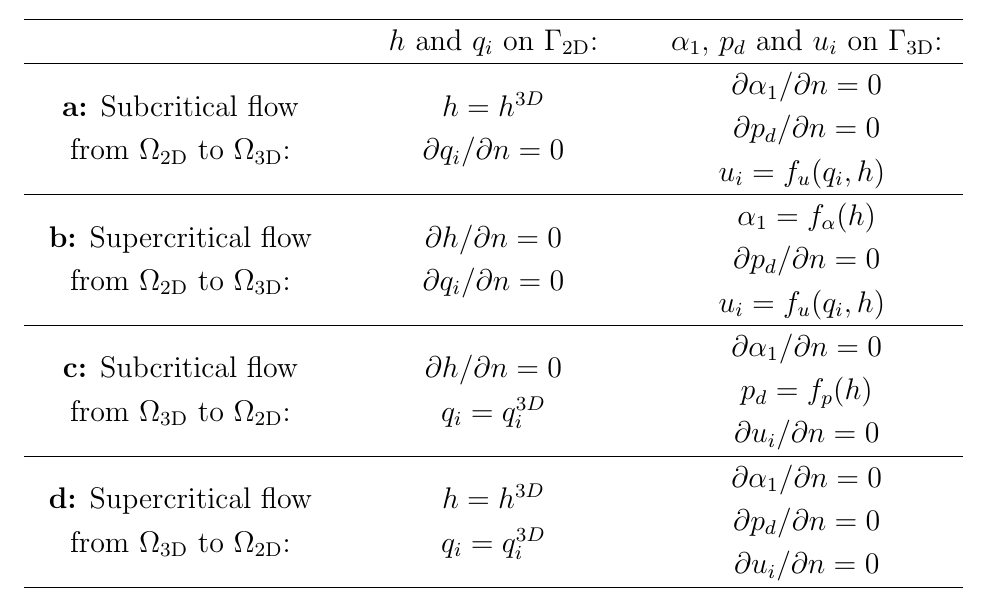
\includegraphics[scale=0.44]{./Resources/Images/bcs_mintgen.png}
\caption{Boundary condition used by \cite{mintgen}}
\end{figure}
\end{frame}

%%%%%%%%%%%%%%%%%%
%%%%%%%%%%%%%%%%%%
\begin{frame}
\shiftedframetitle{Current Status}
\vspace{-0.5cm}
{\large $2D$ SWE - $2D$ SWE \textbf{\myTUMdarkblue{Unidirectional}}}\\
Case: Radial dam break, no bathymetry
\begin{textblock*}{1cm}(17cm,1pt) % {block width} (coords)
%\begin{figure}
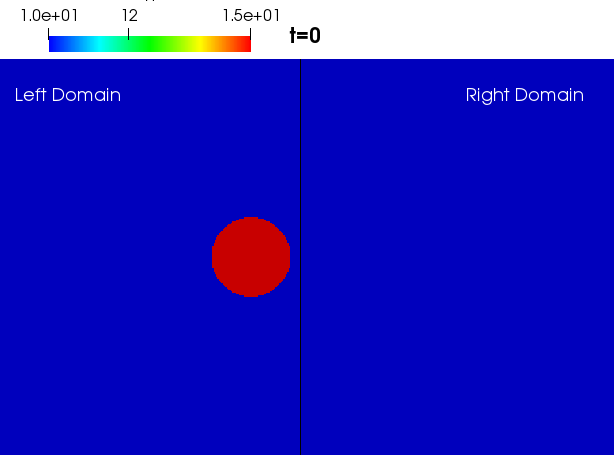
\includegraphics[scale=0.22]{./Resources/Images/unidirectional0_g_0.png}
%\caption{sadf}
%\end{figure}
\end{textblock*}

\begin{figure}[htp]
\centering
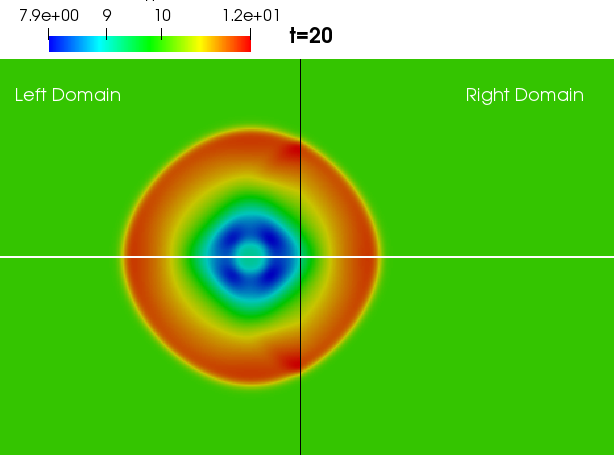
\includegraphics[width=.25\textwidth]{./Resources/Images/unidirectional20_g_0.png}\hfill
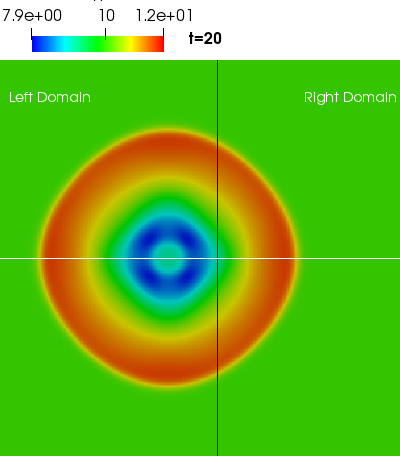
\includegraphics[width=.25\textwidth]{./Resources/Images/unidirectional20_g_bueno.png}\hfill
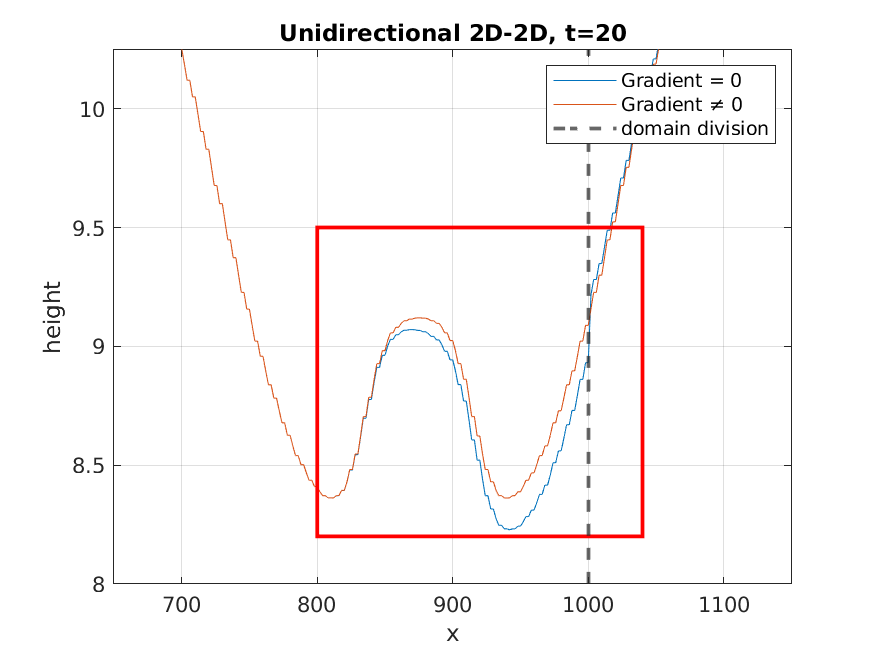
\includegraphics[width=.4\textwidth]{./Resources/Images/unidirectional_graph.png}

\caption{Top right: $h(t=0)$. Left: $h(t=20), \nabla_\eta=0$. Middle: $h(t=20),\nabla_\eta \neq0$. Right: graphed values at the middle of the domain}
\end{figure}

\end{frame}


%%%%%%%%%%%%%%%%%%
%%%%%%%%%%%%%%%%%%
\begin{frame}
\shiftedframetitle{Current Status}
\vspace{-0.5cm}
{\large $2D$ SWE - $2D$ SWE \textbf{\myTUMdarkblue{Bidirectional}}}\\
Case: Radial dam break, no bathymetry
\begin{textblock*}{1cm}(17cm,1pt) % {block width} (coords)
%\begin{figure}
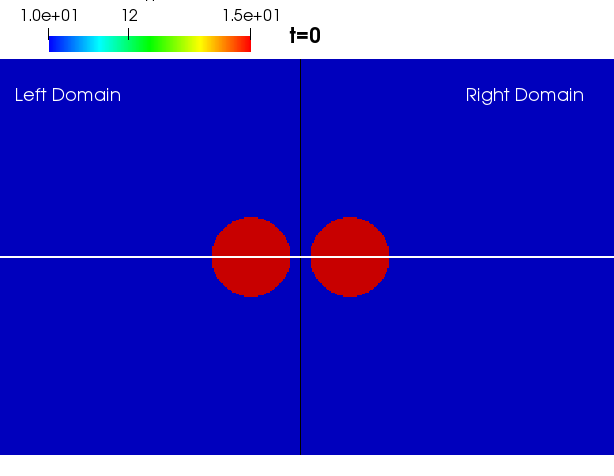
\includegraphics[scale=0.22]{./Resources/Images/bidirectional0_g_0.png}
%\caption{sadf}
%\end{figure}
\end{textblock*}

\begin{figure}[htp]
\centering
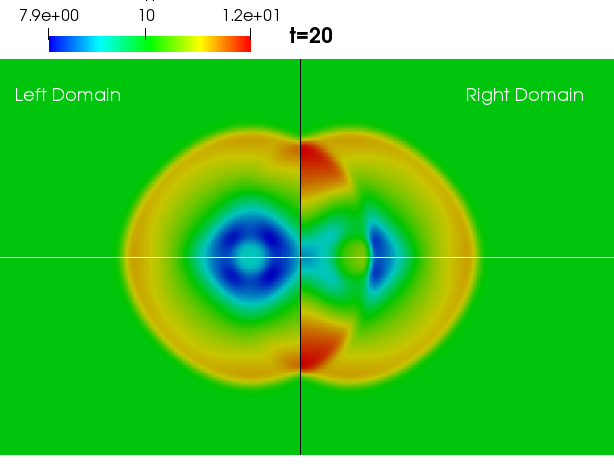
\includegraphics[width=.25\textwidth]{./Resources/Images/bidirectional20_g_0.png}\hfill
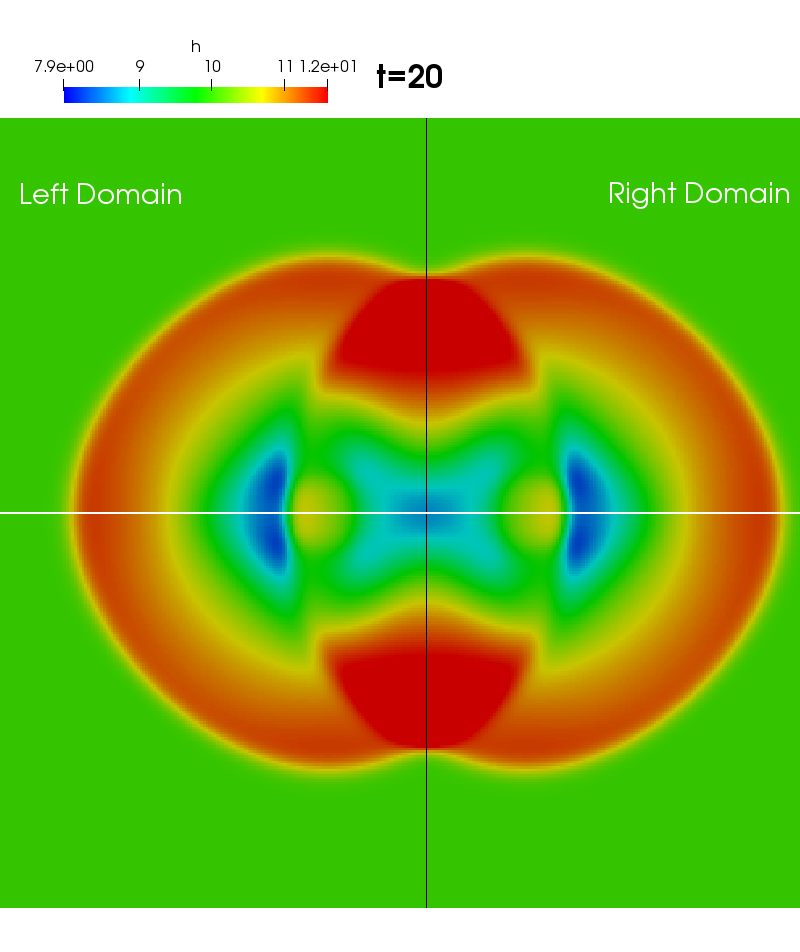
\includegraphics[width=.25\textwidth]{./Resources/Images/bidirectional20_g_bueno.png}\hfill
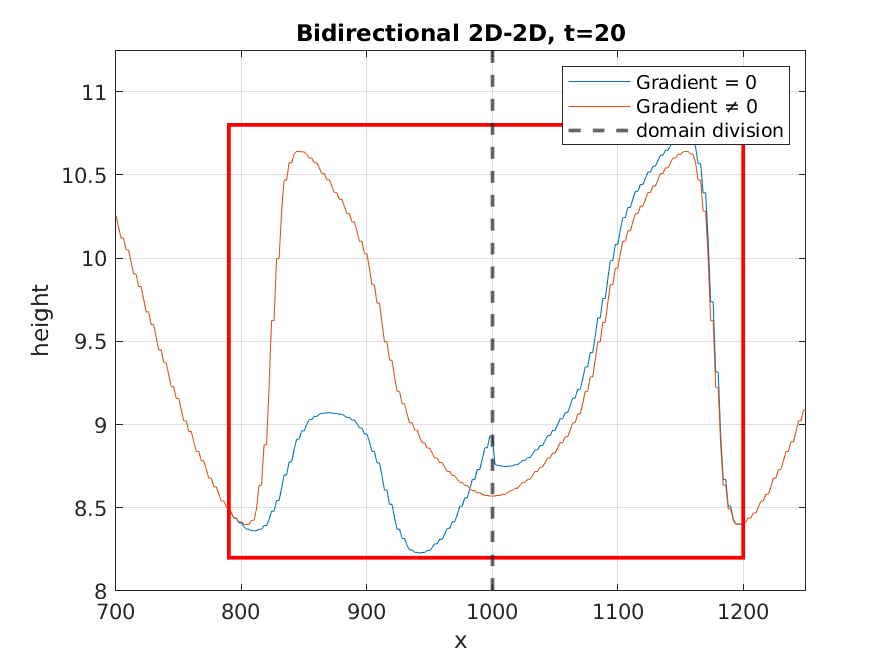
\includegraphics[width=.4\textwidth]{./Resources/Images/bidirectional_graph.png}
\caption{Top right: $h(t=0)$. Left: $h(t=20),\nabla_\eta=0$. Middle: $h(t=20)$,$\nabla_\eta \neq0$. Right: graphed values at the middle of the domain}
\end{figure}

\end{frame}


%%%%%%%%%%%%%%%%%%
%%%%%%%%%%%%%%%%%%
\begin{frame}
\shiftedframetitle{Next steps}
\vspace{-2mm}
{\large Unidirectional Cases}\\
\begin{multicols}{2}
\begin{itemize}
\setlength\itemsep{2em}
\item \myTUMgreen{2D SWE} domain $\leftrightarrow$ \myTUMgreen{3D interFOAM } domain
\item fit \myTUMgreen{Fluid-Fluid adapter} preCICE
\item \myTUMgreen{Exchange} of variables
\begin{itemize}
\setlength\itemsep{1em}
\vspace{5pt}
\item discharges $hu, hv$
\item height $h$
\item volume indicator $\alpha$
\item \myTUMgreen{BCs} $->$ Dirchlet? Neumann? Robin?
\end{itemize}
\end{itemize}

\vfill\columnbreak

\begin{figure}
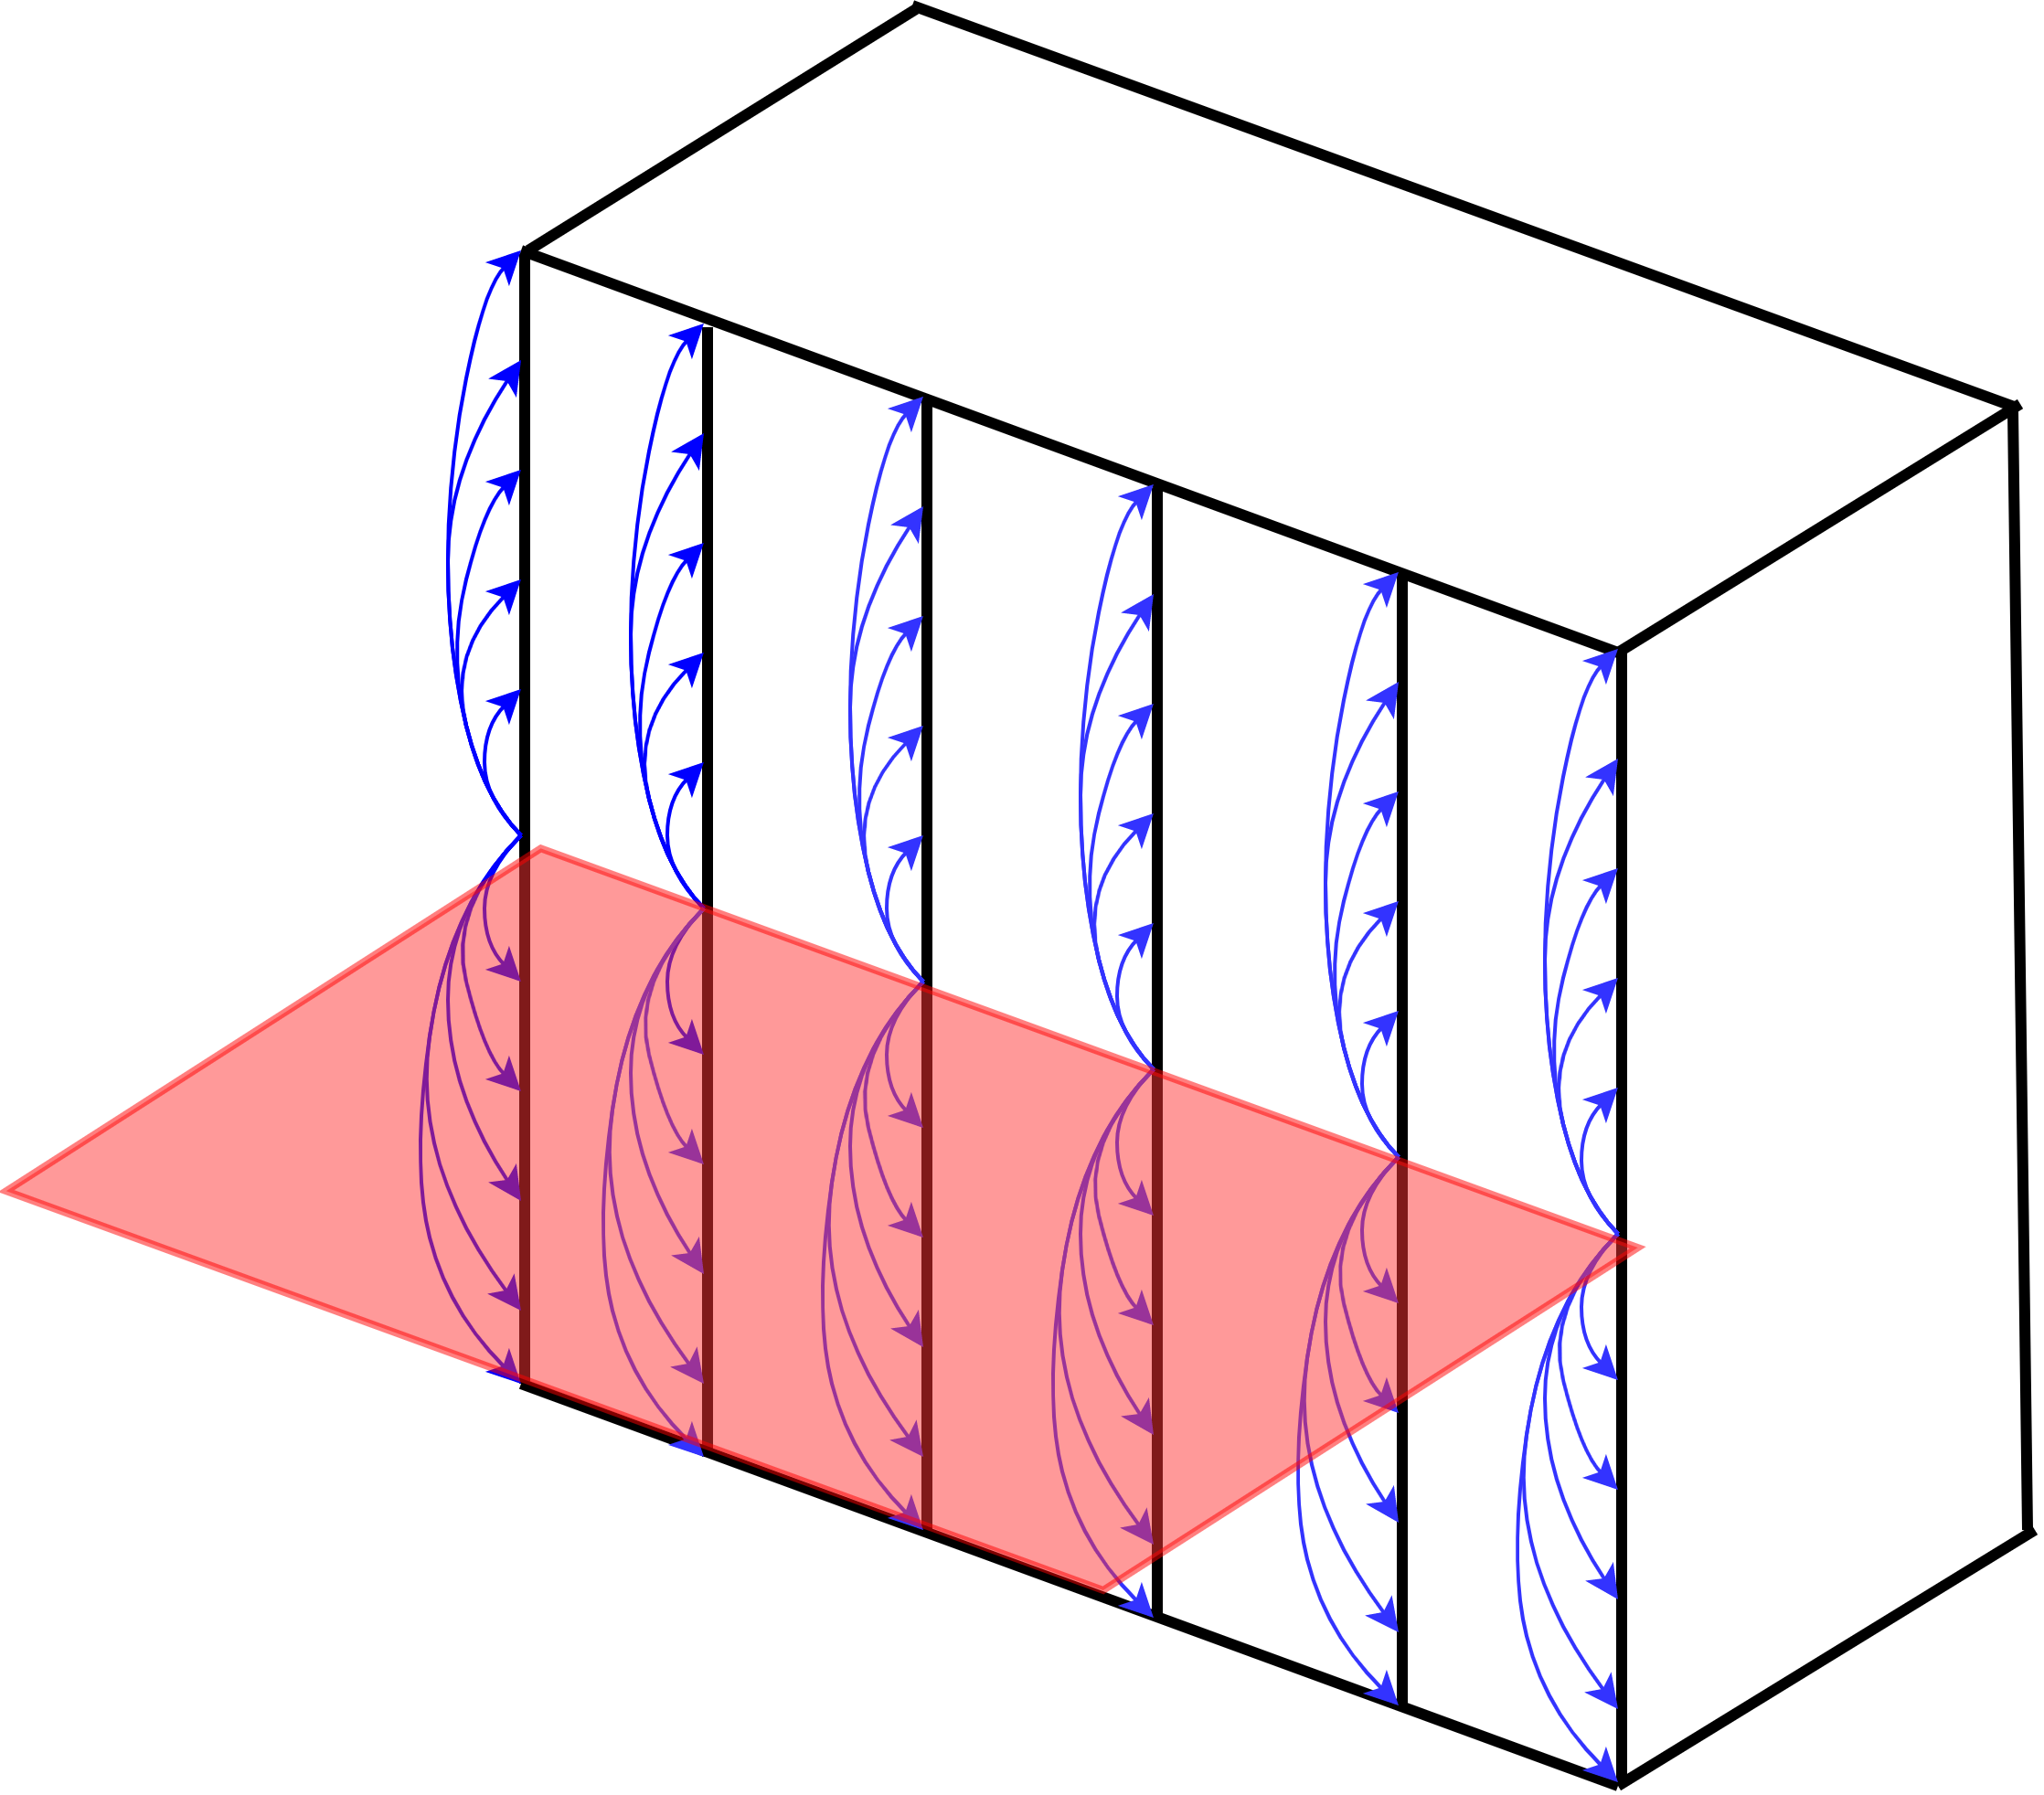
\includegraphics[scale=0.4]{./Resources/Images/mapping23.png}
\\
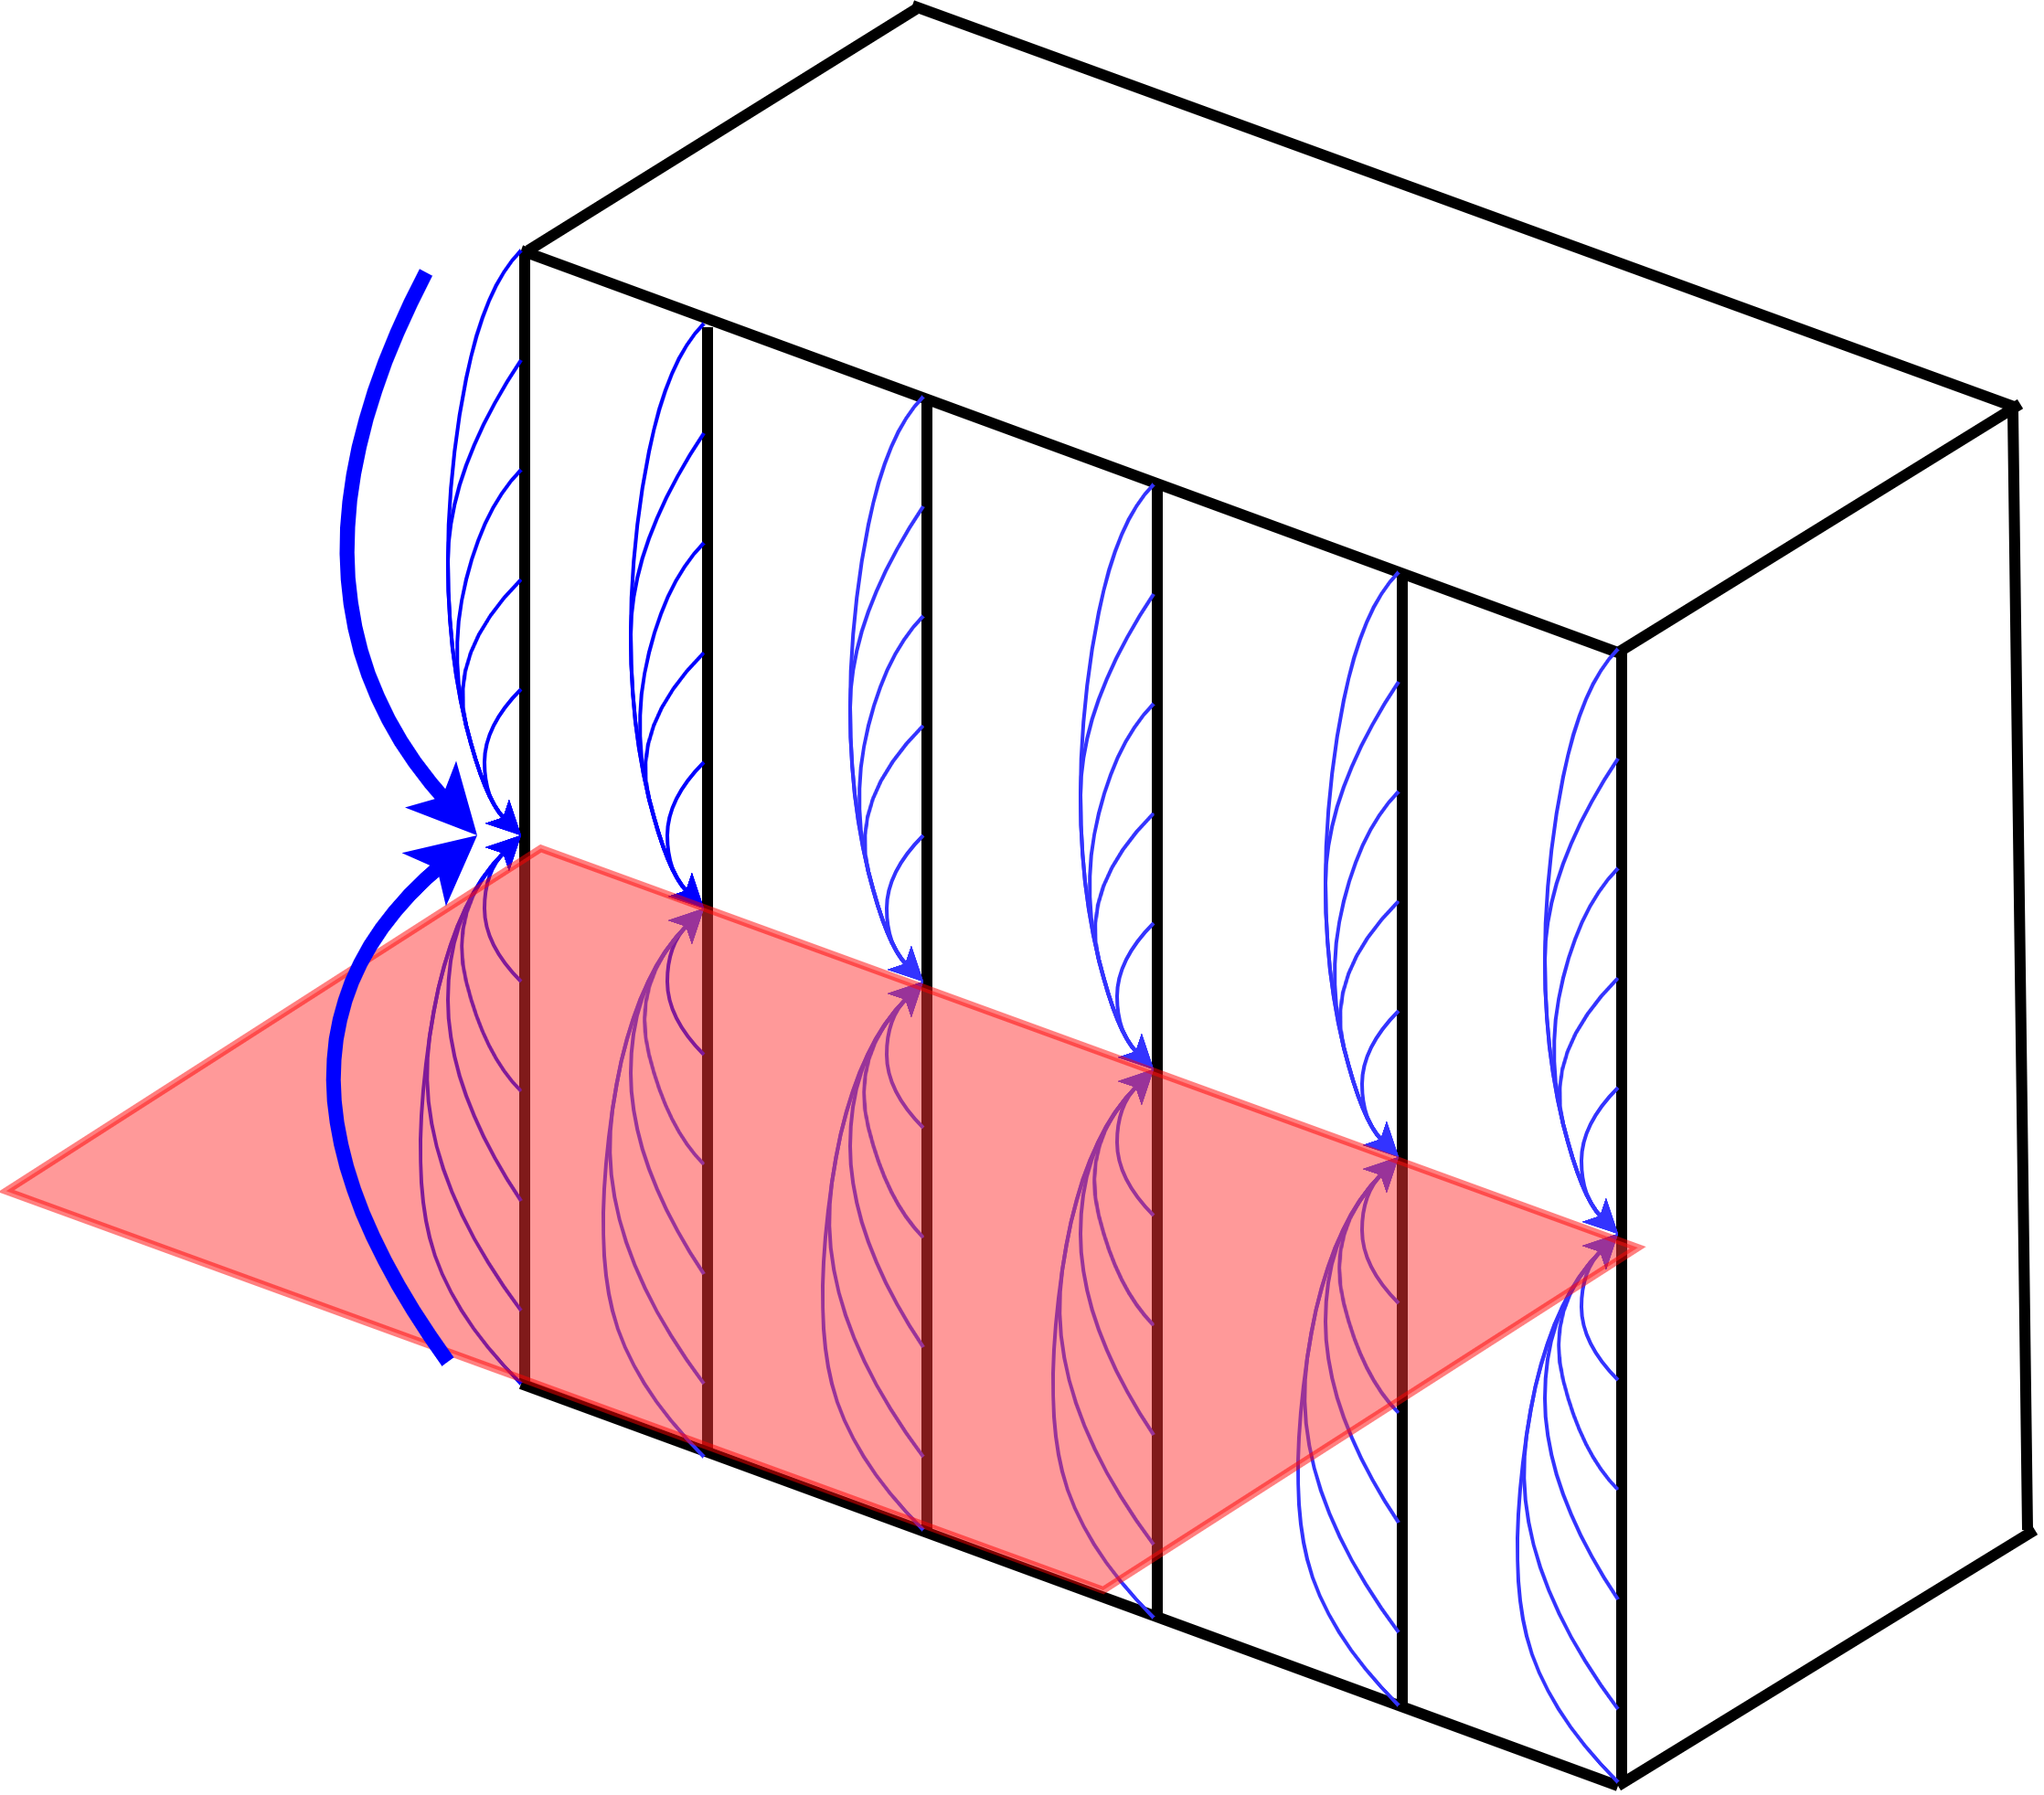
\includegraphics[scale=0.4]{./Resources/Images/mapping32.png}

%\caption<1>{mapping $2D$ to $3D$}
%\caption<2>{mapping $3D$ to $2D$}
\end{figure}

\end{multicols}

\end{frame}


%%%%%%%%%%%%%%%%%%
%%%%%%%%%%%%%%%%%%
\begin{frame}
\shiftedframetitle{Next steps}
\vspace{-2mm}
{\large Bidirectional $3D$}\\
\begin{multicols}{2}
\begin{itemize}
\setlength\itemsep{2em}
\item 3D interFOAM  \textit{left} $\leftrightarrow$ \textit{right} domains
\item fit \myTUMgreen{Fluid-Fluid adapter} preCICE
\item \myTUMgreen{Exchange} of variables
\begin{itemize}
\setlength\itemsep{1em}
\vspace{5pt}
\item discharges $hu, hv$
\item height $h$
\item volume indicator $\alpha$
\item \myTUMgreen{BCs} $->$ Dirchlet? Neumann? Robin?
\end{itemize}
\end{itemize}

\vfill\columnbreak

\begin{figure}
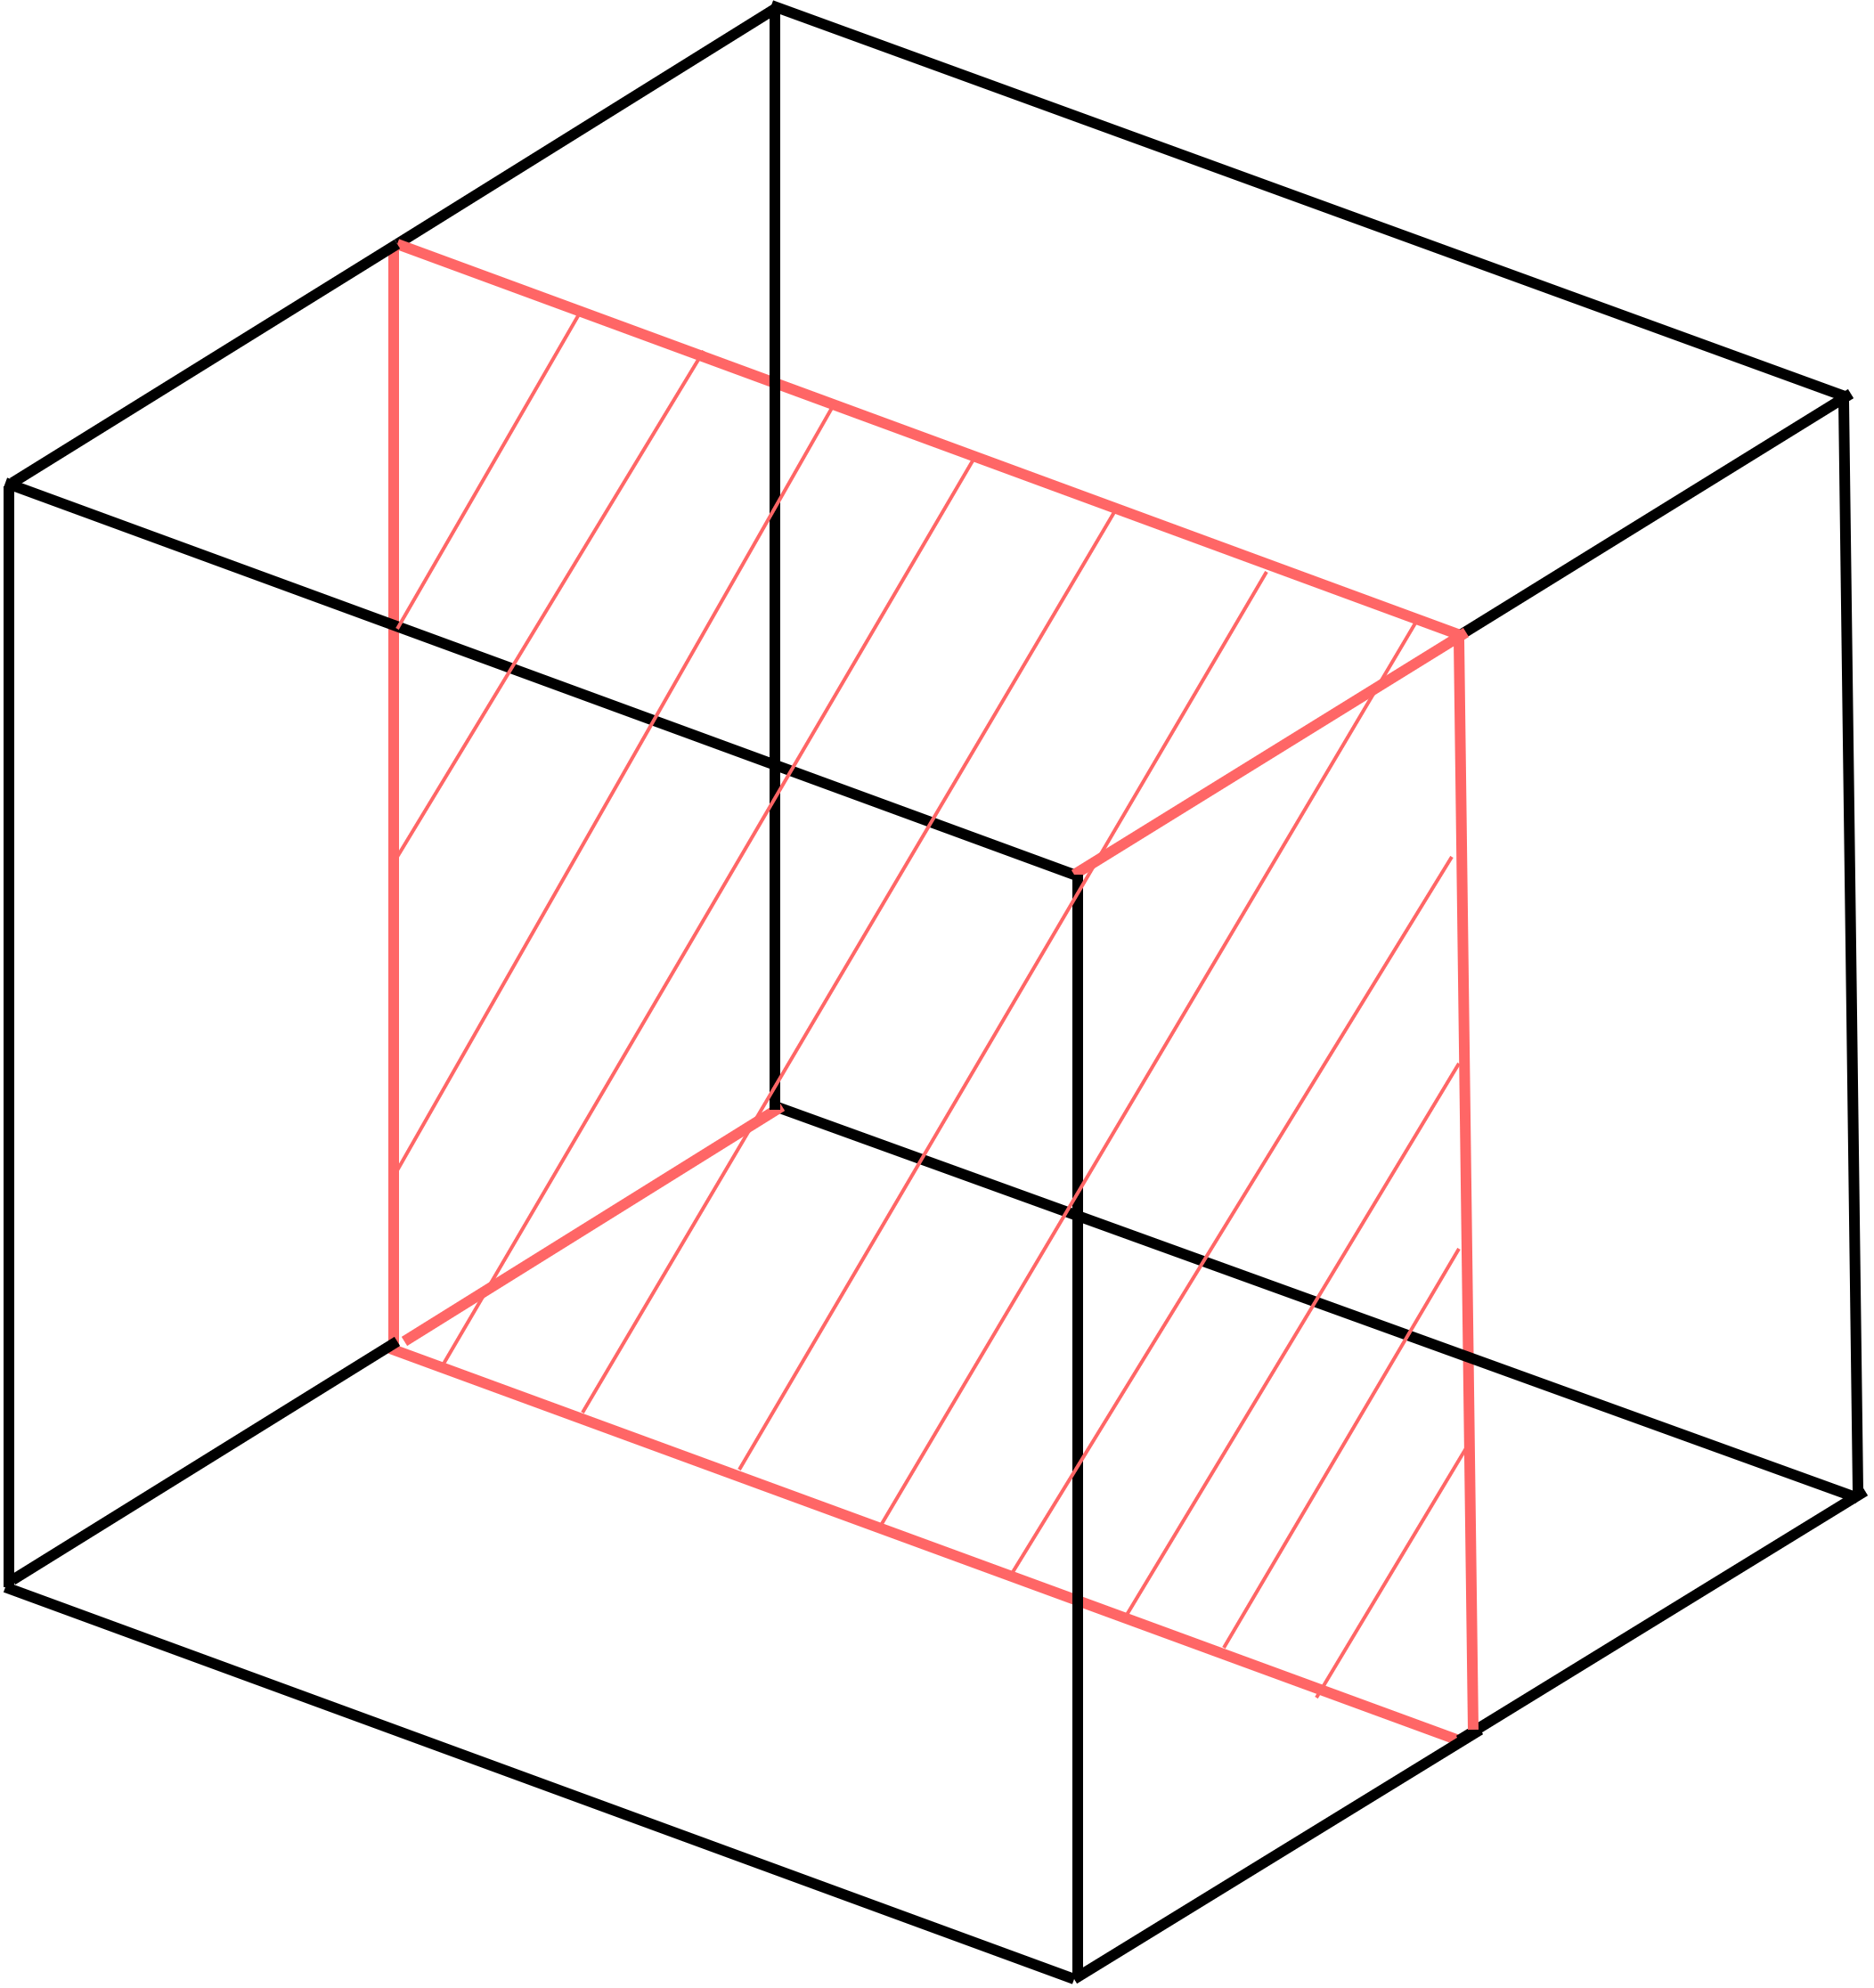
\includegraphics[scale=0.5]{./Resources/Images/mapping33.png}
%\caption<1>{mapping $2D$ to $3D$}
%\caption<2>{mapping $3D$ to $2D$}
\end{figure}

\end{multicols}

\end{frame}



%%%%%%%%%%%%%%%%%%%%
%%% Folie: Farben %%
%%%%%%%%%%%%%%%%%%%%
%\begin{frame}
%    \shiftedframetitle{Farben}
%
%Als erstes soll mit schwarz und weiß gearbeitet werden.\newline
%Für Aufwändigere Darstellungen sind Farben mit Bedacht und in möglichst
%geringem Umfang einzusetzen.
%
%In diesem Folienmaster ist die Farbpalette festgelegt.
%
%{
%    \renewcommand{\arraystretch}{1.2} % skaliert die Tabellen mit Farbfeldern
%
%    Zuerst mit den Primärfarben arbeiten.
%
%    \setlength{\fboxsep}{-1pt} \setlength{\fboxrule}{1pt} % fbox/framebox konfigurieren
%
%    \vspace*{-5mm}
%    \begin{tabularx}{\textwidth}{@{} l @{\hspace{4mm}} l @{\hspace{4mm}} l}
%        \crule[TUMBlau]{24mm}{6mm}
%        & \crule[black]{24mm}{6mm}
%        & \fbox{\crule[white]{24mm}{6mm}}
%    \end{tabularx}
%
%    \vspace*{-5mm}
%    Für z.B. komplexe Diagramme stehen noch Sekundärfarben zur Verfügung.
%
%    \vspace*{-5mm}
%    \begin{tabularx}{\textwidth}{@{} l @{\hspace{4mm}} l @{\hspace{4mm}} l @{\hspace{4mm}} l}
%        \crule[TUMBlauDunkel]{24mm}{6mm}
%        & \crule[TUMBlauMittel]{24mm}{6mm}
%        & \crule[TUMBlauHell]{24mm}{6mm}
%        & \crule[TUMGrau]{24mm}{6mm}
%    \end{tabularx}
%
%    \vspace*{-5mm}
%    Bei weiterer Komplexität oder zusätzlichen Markierungen:
%
%    \vspace*{-5mm}
%    \begin{tabularx}{\textwidth}{@{} l @{\hspace{4mm}} l @{\hspace{4mm}} l }
%        \crule[TUMOrange]{24mm}{6mm}
%        & \crule[TUMGruen]{24mm}{6mm}
%        & \crule[TUMElfenbein]{24mm}{6mm}
%    \end{tabularx}
%}
%
%\end{frame}
%\clearpage
%
%
%%%%%%%%%%%%%%%%%%%
%%% Folie: Texte %%
%%%%%%%%%%%%%%%%%%%
%\begin{frame}
%    \shiftedframetitle{Texte}
%
%Kurze und knappe Texte, Fließtexte linksbündig, kein Blocksatz \\[\baselineskip]
%
%Beispiel:\newline
%Tem soluptam, nisi as verum ereprehendam at acculpa quidisq uissit volupta
%tusdant utem as etur, odi odis es doluptiae dem nimaion con nossinctenis pora
%quam voloria consenimus blabore everfer epeliquo maio etur.
%
%\end{frame}
%\clearpage
%
%
%
%
%%%%%%%%%%%%%%%%%%%%%%%%%%%%%%%
%% Folie: Bilder - Allgemein %%
%%%%%%%%%%%%%%%%%%%%%%%%%%%%%%%
%\begin{frame}
%    \shiftedframetitle{Bilder -- Allgemein}
%
%schlichte Darstellung von Informationen \\[\baselineskip]
%
%reduzierte Farben \\[\baselineskip]
%
%Rahmen und Überlagerungen nach Möglichkeit vermeiden \\[\baselineskip]
%
%
%\end{frame}
%\clearpage
%
%
%%%%%%%%%%%%%%%%%%%%%%%%%%
%% Folie: Bilder - Zwei %%
%%%%%%%%%%%%%%%%%%%%%%%%%%
%\begin{frame}
%    \shiftedframetitle{Bilder}
%
%Bildbeschreibung\newline
%oberer Bildrand: Begrenzung durch Text\\[\baselineskip]
%
%\mbox{
\includegraphics[height=.5\paperheight, trim=0cm 14cm 0cm 0cm, clip=true]{./Resources/Images/SternenhimmelHochkant.jpg}}%
%\hspace{6.5mm}%
%\mbox{
\includegraphics[height=.5\paperheight, trim=0cm 14cm 0cm 0cm, clip=true]{./Resources/Images/SternenhimmelHochkant.jpg}}
%
%\end{frame}
%\clearpage
%
%
%%%%%%%%%%%%%%%%%%%%%%%%%%%%%%%%%%%%%%%%
%% Folie: Bilder - Zweispaltige Seite %%
%%%%%%%%%%%%%%%%%%%%%%%%%%%%%%%%%%%%%%%%
%\begin{frame}
%    \shiftedframetitle{Bilder}
%
%\begin{multicols}{2}
%    \textbf{Überschrift 2}\newline
%    Hier steht ein einleitender oder beschreibender Fließtext und nach Wunsch
%    eine Aufzählung.
%
%    Punkt 1
%
%    Punkt 2
%
%    Punkt 3
%
%    Punkt 4
%    \vfill\columnbreak
%    
\includegraphics[width=\columnwidth, height=.7\textheight]{./Resources/Images/SternenhimmelHochkant.jpg}%
%\end{multicols}
%
%\end{frame}
%\clearpage
%
%
%%%%%%%%%%%%%%%%%%%%%%%%%%%%%%%
%% Folie: Bilder - Textbreit %%
%%%%%%%%%%%%%%%%%%%%%%%%%%%%%%%
%\begin{frame}
%    \shiftedframetitle{Bilder}
%
%Bildbeschreibung\newline
%oberer Bildrand: Begrenzung durch Text\\[\baselineskip]
%
%
\includegraphics[width=\textwidth, height=.55\textheight]{./Resources/Images/SternenhimmelQuer.jpg}%
%
%\end{frame}
%\clearpage
%
%%%%%%%%%%%%%%%%%%%%%%%%%%%%%%%%%%%%%%%%%%%%%%%%%%
%% Folie: Bilder - seitenbreit mit Beschreibung %%
%%%%%%%%%%%%%%%%%%%%%%%%%%%%%%%%%%%%%%%%%%%%%%%%%%
%\begin{frame}
%    \shiftedframetitle{Bilder}
%
%    Bildbeschreibung\newline
%    oberer Bildrand: Begrenzung durch Text
%
%\vspace*{-3mm}
%\begin{minipage}[t][0cm]{\paperwidth}%
%\hspace*{-\PraesentationSeitenrand}%
%
\includegraphics[width=\paperwidth]{./Resources/Images/SternenhimmelQuer.jpg}
%\end{minipage}
%
%\end{frame}
%\clearpage
%
%%%%%%%%%%%%%%%%%%%%%%%%%%%%%%%%%%%%%%%%%%%%%%%%%%%%%
%% Folie: Nicht Format füllende Bilder %%
%%%%%%%%%%%%%%%%%%%%%%%%%%%%%%%%%%%%%%%%%%%%%%%%%%%%%
%\begin{frame}
%    \shiftedframetitle{Nicht Format füllende Bilder}
%
%    Weißer bzw. transparenter Hintergrund\newline
%    mit genug Freiraum anordnen
%
%
%\begin{textblock*}{0.4\paperwidth}[0,1](0cm, \textheight - \PraesentationSeitenrand)%
%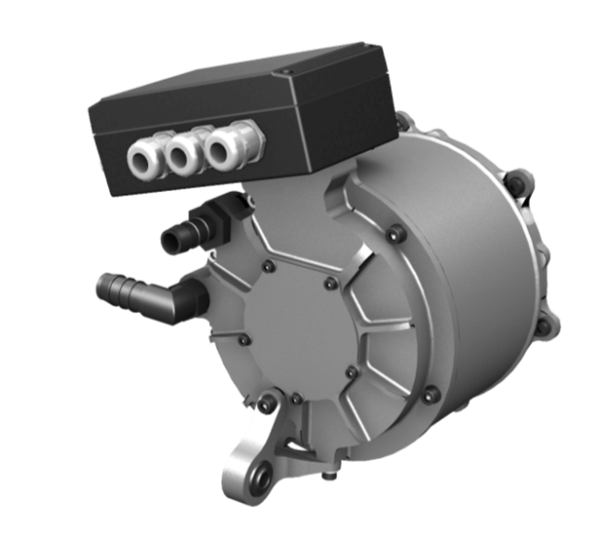
\includegraphics[width=0.4\paperwidth]{./Resources/Presentation/Images/Motor.png}
%\end{textblock*}
%
%\begin{textblock*}{0.6\paperwidth}[1,1](\textwidth + \PraesentationSeitenrand, \textheight - \PraesentationSeitenrand)%
%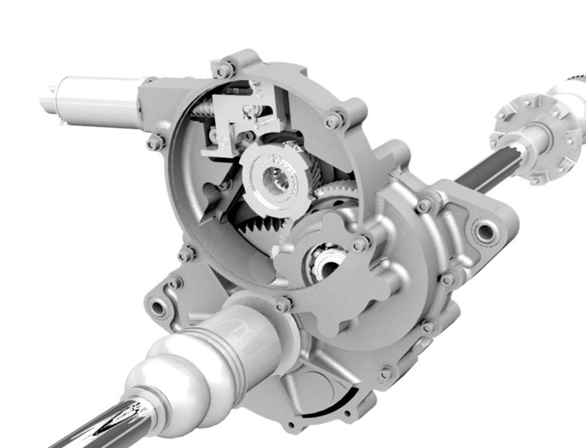
\includegraphics[width=0.6\paperwidth]{./Resources/Presentation/Images/Getriebe.png}
%\end{textblock*}
%
%\end{frame}
%\clearpage
%
%
%%%%%%%%%%%%%%%%%%%%%%%%%%%%%%%%%%%
%% Folie: Bilder - formatfüllend %%
%%%%%%%%%%%%%%%%%%%%%%%%%%%%%%%%%%%
%\begin{frame}
%    \shiftedframetitle{Bilder Format füllend -- maximale Bildgröße}
%
%\begin{minipage}[t][0cm]{\paperwidth}%
%\hspace*{-\PraesentationSeitenrand}%
%
\includegraphics[width=\textwidth]{./Resources/Images/SternenhimmelQuer.jpg}
%\end{minipage}
%
%\end{frame}
%\clearpage
%
%%%%%%%%%%%%%%%%%%%%%%%%%%%%%%%%%%%%%%%%%%%%%%%%%%%%%%
%%% Folie: Nicht Format füllende Bilder %%
%%%%%%%%%%%%%%%%%%%%%%%%%%%%%%%%%%%%%%%%%%%%%%%%%%%%%%
%\begin{frame}
%    \shiftedframetitle{Nicht Format füllende Bilder}
%
%Alternativ mit formatfüllendem Hintergrund: Weiß 5\% dunkler\newline
%Beschriftungen können zusätzlich neben den Bildern angebracht werden
%
%\begin{textblock*}{\paperwidth}[0,0](0cm, .4\textheight)%
%Bilderklärung
%\end{textblock*}
%
%\begin{textblock*}{\paperwidth}[1,0](\textwidth, .4\textheight)%
%\raggedleft%
%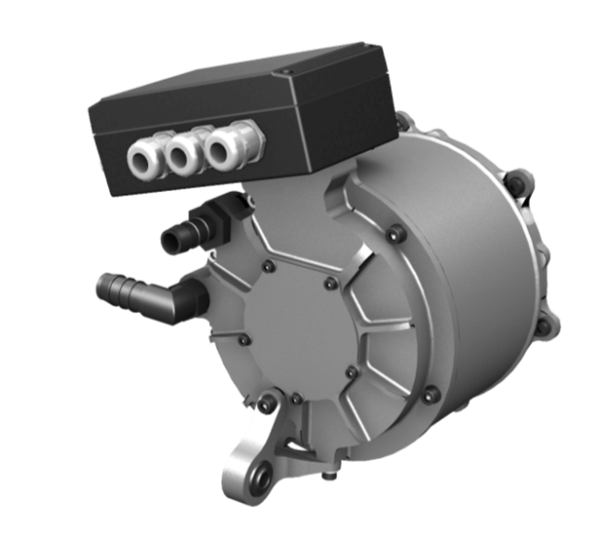
\includegraphics[height=0.5\textheight]{./Resources/Presentation/Images/Motor.png}
%\end{textblock*}
%
%\end{frame}
%\clearpage
%
%
%%%%%%%%%%%%%%%%%%%%%%%%%%%%%%%%%%%%%%%%%%%%%%%%%%%%%
%% Folie: Tabelle - Ohne Rand 					   %%
%%%%%%%%%%%%%%%%%%%%%%%%%%%%%%%%%%%%%%%%%%%%%%%%%%%%%
%\begin{frame}
%    \shiftedframetitle{Tabelle -- Beispiel 1}
%
%Tabelle ohne Farbe und kein Rand \\
%innerer Seitenrand links 0 cm, um Faktor 1,75 skalierte Tabelle (für genug Zeilenabstand)
%
%\raggedright
%{
%    \vspace*{0.3pt}
%    \renewcommand{\arraystretch}{1.75} % skaliert die Tabelle auf die gewünschte Größe
%    \begin{tabularx}{\textwidth}{@{} l @{\hspace{38.7mm}} l}
%        Ø - Strecke & 39 km/Tag (14.360 km/Jahr) \\
%        Ø - Geschwindigkeit & 25 km/h \\
%        Ø - Verfügbare Ladezeit & 22 h/Tag \\
%        Kosten   & Kleinwagen mit Verbrennungsmotor \\
%        Einsatzgebiet   &  Stadt und Umland
%    \end{tabularx}
%}
%\end{frame}
%
%
%%%%%%%%%%%%%%%%%%%%%%%%%%%%%%%%%%%%%%%%%%%%%%%%%%%%%%
%%% Folie: Tabelle - Mit Rand                       %%
%%%%%%%%%%%%%%%%%%%%%%%%%%%%%%%%%%%%%%%%%%%%%%%%%%%%%%
%\begin{frame}
%    \shiftedframetitle{Tabelle -- Beispiel 2}
%
%Tabelle ohne Farbe und mit Rand\\
%automatische Zelleninnenabstände, um Faktor 1,75 skalierte Tabelle (für genug Zeilenabstand)
%
%\raggedright
%{
%    \vspace*{0.3pt}
%    \renewcommand{\arraystretch}{1.75} % skaliert die Tabelle auf die gewünschte Größe
%    \begin{tabularx}{\textwidth}{| l @{\hspace{38.7mm}} | X |}
%        \hline
%        Ø - Strecke & 39 km/Tag (14.360 km/Jahr) \\ \hline
%        Ø - Geschwindigkeit & 25 km/h \\ \hline
%        Ø - Verfügbare Ladezeit & 22 h/Tag \\ \hline
%        Kosten   & Kleinwagen mit Verbrennungsmotor \\ \hline
%        Einsatzgebiet   &  Stadt und Umland \\ \hline
%    \end{tabularx}
%}
%\end{frame}
%
%\clearpage
%
%
%%%%%%%%%%%%%%%%%%%%%%%%%%%%%%%%%%%%%%%%%%%%%%%%%%%%%%
%%% Folie: Diagramme - Beispiel 1                   %%
%%%%%%%%%%%%%%%%%%%%%%%%%%%%%%%%%%%%%%%%%%%%%%%%%%%%%%
%\begin{frame}
%    \shiftedframetitle{Diagramme -- Beispiel 1}
%
%%Nach Möglichkeit linksbündig bleiben \\
%%Unnötige Striche und Balken vermeiden
%
%\begin{center}%
%    \vspace*{-1cm}
%   \begin{tikzpicture}
%        \begin{axis}[
%                % kein Abstand zwischen Balken:
%                xbar=0,
%                draw opacity=0,
%                bar width=14,
%                axis x line=none,
%                axis line style={transparent},
%                every tick/.style={transparent},
%                xmin=0,
%                width=\textwidth,
%                height=.6\textheight,
%                enlarge y limits=0.15,
%                symbolic y coords={Kategorie 4,Kategorie 3,Kategorie 2,Kategorie 1},
%                ytick=data,
%                legend image code/.code={\draw[draw=none] (0cm,-0.12cm) rectangle (0.29cm,0.17cm);}, % Legenden-Symbol
%                legend columns=3,
%                reverse legend,
%                legend style={
%                    fill=none,
%                    draw=none,
%                    /tikz/every odd column/.append style={column sep=0.07cm}, % Abstand zwischen Legenden-Symbol und Text
%                    /tikz/every even column/.append style={column sep=0.8cm} % Abstand zwischen den Legendeneinträgen
%                 },
%                 legend to name=PraesentationDiagrammHorizontalLegende
%            ]
%
%            \addlegendentry{Datenreihe 3}
%            \addlegendentry{Datenreihe 2}
%            \addlegendentry{Datenreihe 1}
%
%            \addplot[color=TUMBlauMittel, fill=TUMBlauMittel] coordinates {
%                (1.2,Kategorie 1)
%                (1.6,Kategorie 2)
%                (2.2,Kategorie 3)
%                (3.4,Kategorie 4)
%            };
%
%            \addplot[color=TUMBlauHell, fill=TUMBlauHell] coordinates {
%                (1.5,Kategorie 1)
%                (3.0,Kategorie 2)
%                (1.0,Kategorie 3)
%                (2.0,Kategorie 4)
%            };
%
%            \addplot[color=TUMBlauDunkel, fill=TUMBlauDunkel] coordinates {
%                (3.0,Kategorie 1)
%                (2.0,Kategorie 2)
%                (2.5,Kategorie 3)
%                (3.0,Kategorie 4)
%            };
%        \end{axis}
%    \end{tikzpicture}
%
%    \vspace*{-5mm}
%    \ref*{PraesentationDiagrammHorizontalLegende}%
%\end{center}
%\end{frame}
%\clearpage
%
%
%%%%%%%%%%%%%%%%%%%%%%%%%%%%%%%%%%%%%%%%%%%%%%%%%%%%%%
%%% Folie: Diagramme                                %%
%%%%%%%%%%%%%%%%%%%%%%%%%%%%%%%%%%%%%%%%%%%%%%%%%%%%%%
%\begin{frame}
%    \shiftedframetitle{Diagramme}
%
%\begin{center}
%    \begin{tikzpicture}
%        \begin{axis}[
%                ybar=9.5,
%                bar width=27.1,
%                axis line style={transparent},
%                every tick/.style={transparent},
%                enlarge x limits=0.145, % X-Achse skalieren
%                clip limits=true,
%                ymin=0,
%                ymax=6,
%                width=\textwidth,
%                height=.65\textheight,
%                symbolic x coords={Kategorie 1,Kategorie 2,Kategorie 3,Kategorie 4},
%                xticklabels={Kategorie 1,Kategorie 2,Kategorie 3,Kategorie 4},
%                xtick=data,
%                ytick={0,1,2,3,4,5,6},
%                every tick label/.append style={font=\fontsize{13}{14}\selectfont},
%                ymajorgrids,
%                legend image code/.code={\draw[draw=none] (0cm,-0.12cm) rectangle (0.29cm,0.17cm);}, % Legenden-Symbol
%                legend columns=3,
%                reverse legend,
%                legend style={
%                    font={\usebeamerfont{footnote}},
%                    fill=none,
%                    draw=none,
%                    /tikz/every odd column/.append style={column sep=0.07cm}, % Abstand zwischen Legenden-Symbol
%                    /tikz/every even column/.append style={column sep=0.8cm} % Abstand zwischen den Legendeneinträgen
%                 },
%                legend to name=PraesentationDiagrammVertikalLegende
%            ]
%
%            \addlegendentry{Datenreihe 3}
%            \addlegendentry{Datenreihe 2}
%            \addlegendentry{Datenreihe 1}
%
%            \addplot[color=TUMBlauDunkel, fill=TUMBlauDunkel] coordinates {
%                (Kategorie 1,4.2)
%                (Kategorie 2,2.5)
%                (Kategorie 3,3.5)
%                (Kategorie 4,4.5)
%            };
%
%            \addplot[color=TUMBlauHell, fill=TUMBlauHell] coordinates {
%                (Kategorie 1,2.3)
%                (Kategorie 2,4.5)
%                (Kategorie 3,1.8)
%                (Kategorie 4,2.8)
%            };
%
%            \addplot[color=TUMBlauMittel, fill=TUMBlauMittel] coordinates {
%                (Kategorie 1,2.0)
%                (Kategorie 2,2.0)
%                (Kategorie 3,3.0)
%                (Kategorie 4,5.0)
%            };
%        \end{axis}
%    \end{tikzpicture}
%
%    \vspace*{-5mm}
%    \ref*{PraesentationDiagrammVertikalLegende}%
%\end{center}
%\end{frame}
%\clearpage
%
